\begin{frame}[noframenumbering]
	\centering
	\huge Our Adaptive SPS \\ Reactive approach (RA-SPS)
\end{frame}


\begin{frame}{Reactive approach : RA-SPS}
	\begin{block}{Proposal}
	Analyse the \textbf{operator state} to modify the number of active replicas of the operators in the DAG		
	\end{block}
\end{frame}

\begin{frame}{Reactive approach : RA-SPS}
	State metric $\delta$ is a multi-metric based in : 
	\begin{itemize}
		\item Utilization (U) : Operator load
		\item Execution time (E) : Degradation execution time
		\item Queue (Q) : Impact of queue size
	\end{itemize}
	\vspace*{0.5cm}	
	Each metric is discrete and calculated according to the time interval $t$
	\vspace*{-2.5cm}
	\begin{figure}
		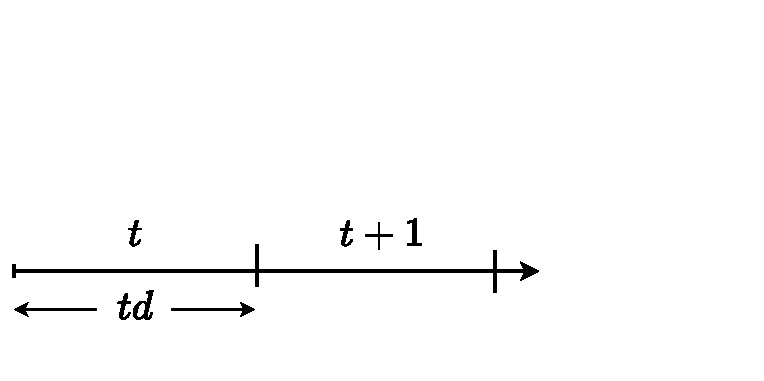
\includegraphics[scale=0.75]{images/concepts/Interval.pdf}
	\end{figure}
\end{frame}

\begin{frame}{Reactive approach : RA-SPS}
	\textbf{Utilisation metric}\\
	\vspace*{0.2cm}
	Percentage of time that the operator $O_i$ is processing during $t$
	\begin{align*}
        U_i(t) = \frac{\mu_i(t) \times et_i(t)}{r_i(t) \times td}
   	\end{align*}   	
%   	\begin{tabular}{r l}
%   	$\mu_i(t)$ & number of events processed by operator $O_i$ during $t$ \\
%   	${et}_i(t)$ & average execution of one event by operator $O_i$ during $t$ \\
%	$r_i(t)$ & number of active replicas of operator $O_i$ during $t$ \\
%	$td$ & time interval duration \\
%   	\end{tabular}
\end{frame}

\begin{frame}{Reactive approach : RA-SPS}
	\textbf{Utilisation metric}
	\begin{center}
	\begin{align*}
        U_i(t) = \frac{\mu_i(t) \times et_i(t)}{r_i(t) \times td}
   	\end{align*}
   	\vspace*{-1cm}
   	\begin{figure}
   		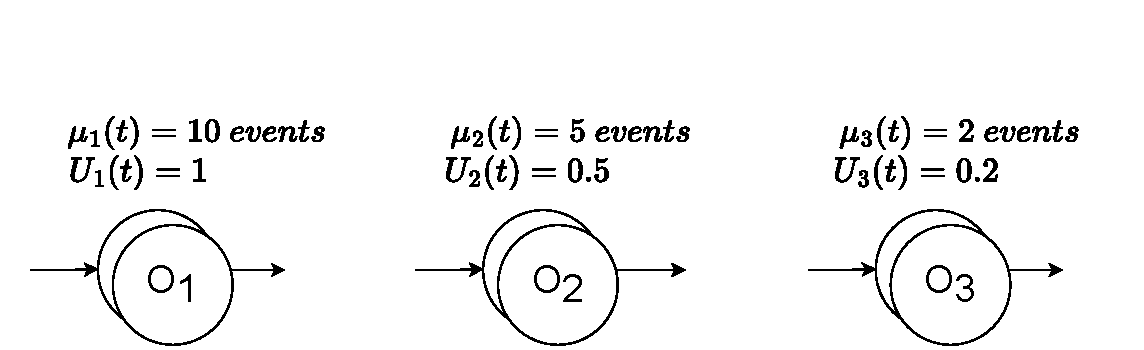
\includegraphics[scale=0.5]{images/concepts/reactive/RA-SPS-Metric-U.pdf}
   	\end{figure}
 	
  	$et_i(t) = 200~ms$ ; $r_i(t) = 2~ms$ ; $td = 1000~ms$ ; $i \in [1,2,3]$
  	\end{center}
\end{frame}
   	
\begin{frame}{Reactive approach : RA-SPS}
	\textbf{Execution time metric}\\
	\vspace*{0.2cm}
	Execution time degradation of the operator $O_i$ during $t$
%	\begin{center}	
   	\begin{align*}
        E_i(t) = 1-\frac{et_i}{et_i(t)}
    \end{align*}
    \vspace*{0.2cm}
    
    \begin{tabular}{r l}
%   	${et}_i(t)$ & average execution of one event by operator $O_i$ during $t$ \\
	${et}_i$ & average execution time of one event by operator $O_i$ \\
	 		 & according to the benchmark\\
   	\end{tabular}
%   	\end{center}
\end{frame}

\begin{frame}{Reactive approach : RA-SPS}
	\textbf{Execution time metric}
	\begin{center}
	\begin{align*}
        E_i(t) = 1-\frac{et_i}{et_i(t)}
   	\end{align*}
   	\vspace*{-0.75cm}
   	\begin{figure}
   		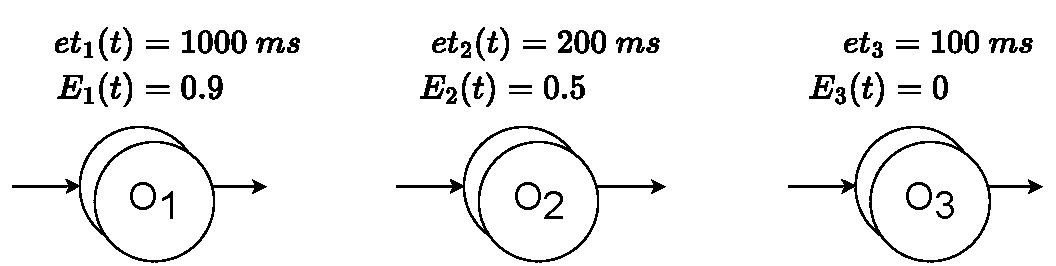
\includegraphics[scale=0.5]{images/concepts/reactive/RA-SPS-Metric-E.pdf}
   	\end{figure}
 	
  	$et_i = 100~ms$ ; $i \in [1,2,3]$
  	\end{center}
\end{frame}
    
\begin{frame}{Reactive approach : RA-SPS}    
	\textbf{Queue metric}\\
	\vspace*{0.2cm}
	Impact of the queue size of the operator $O_i$ according to the processing during $t$
%	\begin{center}
    \begin{align*}
        Q_i(t) = 1-\frac{\mu_i(t)}{q_i(t)}
    \end{align*}
    
%    \begin{tabular}{r l}
%   	$\mu_i(t)$ & number of events processed by operator $O_i$ during $t$ \\
%	$q_i(t)$ & number of events queued by operator $O_i$ during $t$ \\
%   	\end{tabular}
%   	\end{center}
\end{frame}

\begin{frame}{Reactive approach : RA-SPS}
	\textbf{Queue metric}
	\begin{center}
	\begin{align*}
        Q_i(t) = 1-\frac{\mu_i(t)}{q_i(t)}
   	\end{align*}
   	\vspace*{-0.75cm}
   	\begin{figure}
   		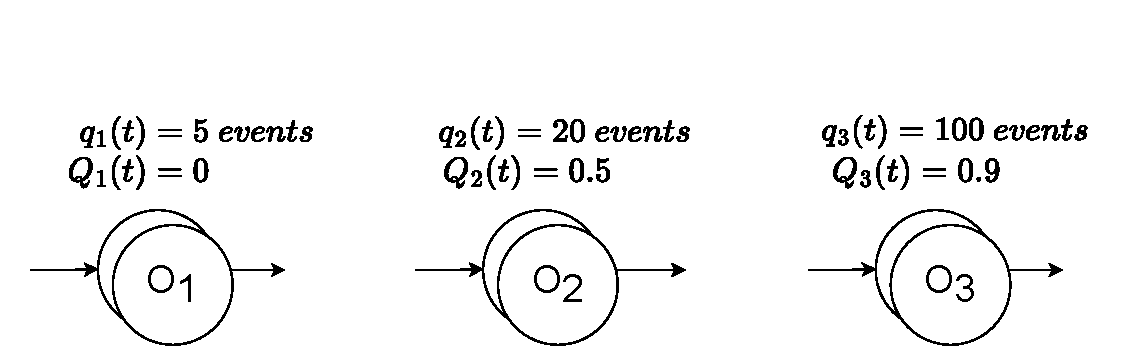
\includegraphics[scale=0.5]{images/concepts/reactive/RA-SPS-Metric-Q.pdf}
   	\end{figure}
 	
  	$\mu_i(t) = 10~events$ ; $i \in [1,2,3]$
  	\end{center}
\end{frame}
	
\begin{frame}{Reactive approach : RA-SPS}
		\textbf{State metric} $\delta_i(t)$ is determined by the three metrics and their respective weights
        \begin{align*}
            \delta_i(t) = U_i(t) \times \omega_U + Q_i(t) \times \omega_Q + E_i(t) \times \omega_E
        \end{align*}   
\end{frame}
	
\begin{frame}{Reactive approach : RA-SPS}
	Analysis of the operator state
		
		\begin{tabular}{l l}
		$\delta_i(t) < \delta_l$ & underloaded \\
		$\delta_l \leq \delta_i(t) \leq \delta_u$ & stable \\
		$\delta_i(t) > \delta_l$ & overloaded
		\end{tabular}
	
	\begin{figure}
		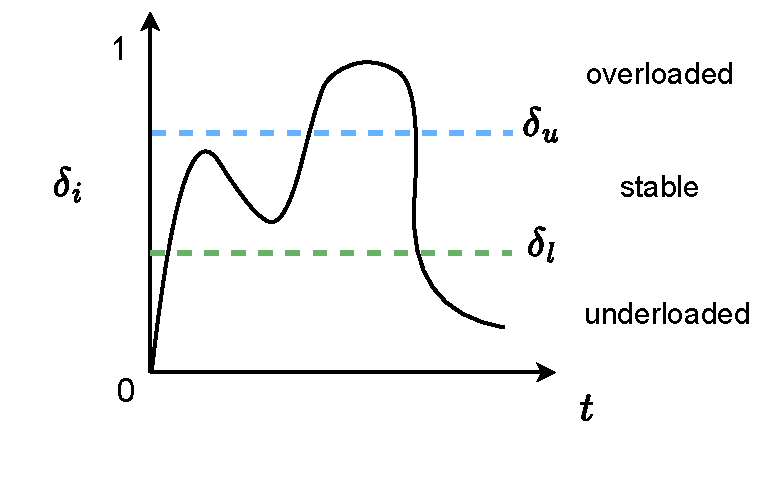
\includegraphics[scale=0.6]{images/concepts/reactive/RA-SPS-Metric-Delta.pdf}
	\end{figure}
\end{frame}

\begin{frame}{Reactive approach : RA-SPS}
    \textbf{Planning algorithm}\\
    \vspace*{0.2cm}
    Analyse if the current state is equal to the precedent state
	\begin{figure}
		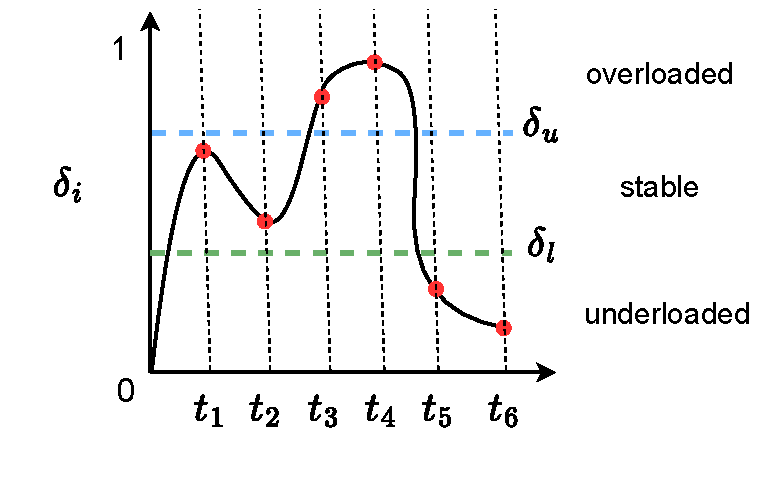
\includegraphics[scale=0.6]{images/concepts/reactive/RA-SPS-Plan.pdf}
	\end{figure}
	\vspace*{-0.2cm}
	\only<1>{
		\textbf{$t_1$}
	}
	
	\only<2>{
		\textbf{$t_2$} : State($\delta_i(t_2)$) $=$ State($\delta_i(t_1)$) ?
	}
	
	\only<3>{
		\textbf{$t_3$} : State($\delta_i(t_3)$) $=$ State($\delta_i(t_2)$) ?
	}
	
	\only<4>{
		
		\textbf{$t_4$} : State($\delta_i(t_4)$) $=$ State($\delta_i(t_3)$) ? Is the machine overloaded ?\\
		 %$E_i(t) > \delta_{E}$ ? \\		
		\textbf{Activate} $k$ replicas of the operator $O_i$
	}
	
	\only<5>{
		\textbf{$t_5$} : State($\delta_i(t_5)$) $=$ State($\delta_i(t_4)$) ?
	}
	
	\only<6>{
		\textbf{$t_6$} : State($\delta_i(t_6)$) $=$ State($\delta_i(t_5)$) ?\\
		\textbf{Deactivate} $k$ replicas of the operator $O_i$
	}
\end{frame}
